% ~~~~~~~~~~~~~~~~~~~~~~~~~~~~~~~~~~~~~~~~~~~~~~~
% ~~~~~~~~~~~~~~ START OF PREAMBLE ~~~~~~~~~~~~~~

\documentclass[12pt]{article}
\usepackage{parskip} % for spacing between paragraphs and eliminating indentation at start of paragraph

\usepackage{tikz-uml}
\usetikzlibrary{
    positioning,
    shapes.geometric,
    arrows,
    arrows.meta,
    }
\usepackage{xspace}
\usepackage{xcolor}
\usepackage{algpseudocodex} % Load the algpseudocodex package

% commands that will be "variables" for the rest of the document
\newcommand\groupname{\textit{Cometical}\xspace}
\newcommand\groupnumber{\textit{24}\xspace}
\newcommand\app{\textit{Assignment and Study Tracker} app\xspace}
\newcommand\classname{\textit{CS 1200.005}\xspace}
\newcommand\assignment{\textit{Deliverable 3}\xspace}

% Place header for first page
\usepackage{fancyhdr}
\fancypagestyle{plain}{} % plain for first page
\fancyhf{}
\fancyhead[L]{\assignment}
\fancyhead[R]{\classname}

% Title 
\title{
    \textbf{Develop by Diego R.R.} \\
    \groupname \\
    \small{group} \# \groupnumber \\
}

% Group members, this is part of the title page
\author{
    \textbf{Diego R.R.} \\
    \texttt{dar220007@utdallas.edu} \\
    \and 
    \textbf{Gael Romero} \\
    \texttt{jgr230000@utdallas.edu} \\
    \and
    \textbf{Emily Rouse} \\
    \texttt{zxr220003@utdallas.edu} \\
    \and
    \textbf{Alan Roybal: \underline{leader}} \\
    \texttt{aer220004@utdallas.edu} \\
    \and
    \textbf{Rishabh Sabnavis} \\
    \texttt{rds230002@utdallas.edu}
}

\date{\today} % automatically generate date, part of title

% Setting header for subsequent pages
\pagestyle{fancy}
\fancyhead[L]{\assignment}
\fancyhead[R]{\classname}

% ~~~~~~~~~~~ END OF PREAMBLE ~~~~~~~~~~~
% ~~~~~~~~~~~~~~~~~~~~~~~~~~~~~~~~~~~~~~~


% ~~~~~~~~~~~~~~~~~~~~~~~~~~~~~~~~~~~~~~~
% ~~~~~~~~~~~~ START OF DOCUMENT ~~~~~~~~
\begin{document}
\maketitle % insert titlepage

% start of project description section
\section{Project Idea} 
    We have selected the \app idea for our project. This app is meant as an integrative solution, designed for students who are struggling with multiple responsibilities and deadlines.
% end of project description

% SUBSYSTEMS
\newcommand\subsystem{Scheduling and Planning Subsystem\xspace}
\newcommand\dataSubsystem{Data Integration and Synchronization Subsystem\xspace}
\newcommand\alertsSubsystem{Notification, Alerts and Data Interpretation subsystem\xspace}
\newcommand\userSubsystem{User Profile Management and Customization Subsystem\xspace}
\newcommand\securitySubsystem{Security and Privacy Subsystem\xspace}


\section{\subsystem}
    The \subsystem is a core component of the \app, designed to provide a comprehensive solution for managing academic responsibilities. Its primary function is to integrate seamlessly with eLearning platforms, harnessing a variety of data points such as assignment due dates, quiz schedules, test timings, and extracurricular event dates. This integration allows for the creation of a dynamic, customizable scheduling planner that goes beyond mere reminders, actively assisting students in optimizing their time based on their academic and personal commitments.

% name to the intelligent process that will be used to create the schedule
\newcommand\scheduler{\textit{Scheduler}\xspace}

% division into functions
\newcommand\dataRetrieval{\textit{Data Retrieval Function}\xspace}
\newcommand\persoanlizedScheduler{\textit{Personalized Scheduler Function}\xspace}
\newcommand\dynamicScheduler{\textit{Dynamic Scheduler Adjustment Function}\xspace}
\newcommand\userInterface{\textit{User Interaction and Interface Function}\xspace}

\section{Design}
In the \app, the \subsystem is integrated with other subsystems, adhering to the Input, Process, Output design paradigm. The \textbf{Input} phase, led by the \dataRetrieval, works closely with the \dataSubsystem to ensure accurate data collection from eLearning platforms needed for the \scheduler. The \textbf{Process} phase is named \scheduler and is split between the \persoanlizedScheduler and \dynamicScheduler. \persoanlizedScheduler works with \securitySubsystem and \userSubsystem to provide a customizable experience and adhere to the privacy contracts. Finally, the \textbf{Output} phase is encompassed by \userInterface. This cohesive structure ensures that each subsystem not only performs its specific role but also collaboratively contributes to a harmonious and effective overall system.

\subsection{Visual Prototype}
To provide a more comprehensive explanation of why the Scheduling and Planning Subsystem in \app lacks a visual prototype, it's crucial to understand the nature of its operations and design philosophy. This subsystem is fundamentally a backend functionality, focusing on processing and managing academic data retrieved from eLearning. Its primary responsibility is to handle complex tasks such as parsing assignment deadlines, quiz schedules, and other academic events. This emphasis on data processing is a clear indication of its backend orientation, where the main objective is to ensure accurate, efficient, and reliable data handling rather than visual presentation.

\newpage

\subsection{Pseudocode}

\subsubsection{Data Retrieval Function}
Retrieving the ELearningAPI is handled by the \dataSubsystem. The \subsystem only needs to call the \dataSubsystem to retrieve the ELearningAPI. The ELearningAPI is then used to retrieve the calendar and preferences for the user, later used by the hollistic algorithm.
\begin{algorithmic}[1] % The [1] option enables line numbering
\Function{RetrieveDataForScheduling}{$user$}
    \State $eLearn \gets \textbf{new} ELearningAPI$
    \State $calendar \gets eLearn.getCalendar(user)$
    \State $preferences \gets user.getPreferences()$
    \State $schedule \gets \textbf{new} Schedule$
    \State \Comment{New Schedule based on calendar, preferences, and user}
    \State \Comment{This schedule is just the list of events retrieved from eLearning}
    \State \Return $schedule$
\EndFunction
\Statex

\end{algorithmic}

\subsubsection{Personalized Scheduler Function}
This function received the data from the \dataSubsystem and generates a personalized schedule for the user. The initialization of the scheduler consist of algorithm that checks multiple conflicts such as privacy hints and personal preferences.
\begin{algorithmic}[1] % The [1] option enables line numbering
\Function{PersonalizedScheduler}{$user$}
    \State $schedule \gets$ \Call{retrieveDataForScheduling}{$user$}
    \State $personalizedSchedule \gets new\ Schedule$
    \ForAll {$event \textbf{ in } schedule.getEvents()$}
        \If {\Call{IsConflict}{$event$, $personalizedSchedule$}}
            \State $event \gets$ \Call{ResolveConflict}{$event$, $personalizedSchedule$}
        \EndIf
        \State \Call{ApplyPreferencesToEvent}{$event$, $user.getPreferences()$}
        \State $personalizedSchedule$.addEvent($event$)
    \EndFor
    \State \Return $personalizedSchedule$
\EndFunction
\Statex

\Function{ApplyPreferencesToEvent}{$event$, $preferences$}
    \ForAll {$preference \textbf{ in } preferences$}
        \State \Comment{Modify the event based on the preference}
        \State \Comment{This would be a family of functions that modify the event}
    \EndFor
    \State \Return $event$
\EndFunction
\Statex

\Function{IsConflict}{$event$, $schedule$}
    \ForAll {$scheduledEvent \textbf{ in } schedule.getEvents()$}
        \If {\Call{IsOverlapping}{$event$, $scheduledEvent$}}
            \State \Comment{Implementation of IsOverlapping exluded for brevity}
            \State \Return $\textbf{true}$
        \EndIf
    \EndFor
    \State \Return $\textbf{false}$
\EndFunction
\Statex

\Function{ResolveConflict}{$event$, $schedule$}
    \State \Comment{Ask user for input on how to resolve the conflict}
    \State \Comment{Resolve problem and retrieve new event}
    \State \Return $event$
\EndFunction
\Statex

\end{algorithmic}

\subsubsection{Dynamic Scheduler Adjustment Function}
Machine intelligence used for this function was simplified to a hollistic algorithm. Take into account that this is the most independent function from other subsystems and it assumes that the Personalized Scheduler Function initialized the hints correctly.
\begin{algorithmic}[1] % The [1] option enables line numbering
\Function{DynamicScheduler}{$user$, $schedule$, $ELearnAPI$}
    \State $userData \gets$ $ELearnAPI$.getData($user$)
    \State $peerData \gets$ $ELearnAPI$.peerData()
    \While{\textbf{not} \Call{IsEndOfDay}{}}
        \State $performance \gets$ $userData$.getInteger()
        \State $adjustments \gets$ \Call{Hollistic}{$performance$, $peerData$, $schedule$}
        \State \Call{ApplyAdjustments}{$schedule$, $adjustments$}
        \State \Call{OptimizeSchedule}{$schedule$}
        \State \textbf{wait} for a predefined interval
    \EndWhile
    \State \Return $newSchedule$
\EndFunction
\Statex

\Function{Hollistic}{$performance$, $peerData$, $schedule$}
    \State \Comment{Perform analysis on the performance and peer data}
    \State \Comment{Generate adjustments to the schedule}
    \State \Return $adjustments$
\EndFunction
\Statex

\Function{ApplyScheduleAdjustments}{$schedule$, $adjustments$}
    \State \Comment{Apply generated adjustments to the schedule}
\EndFunction
\Statex

\Function{OptimizeSchedule}{$schedule$}
    \State \Comment{Use machine intelligence to further optimize the schedule}
\EndFunction

\end{algorithmic}

\subsubsection{User Interaction and Interface Function}
Since the \subsystem is a backend component, it does not have a user interface. However, it does interact with the \userSubsystem and \securitySubsystem to ensure that the user has a customizable experience and that their privacy is protected.

\newpage
\subsection{UML Activity Diagram}

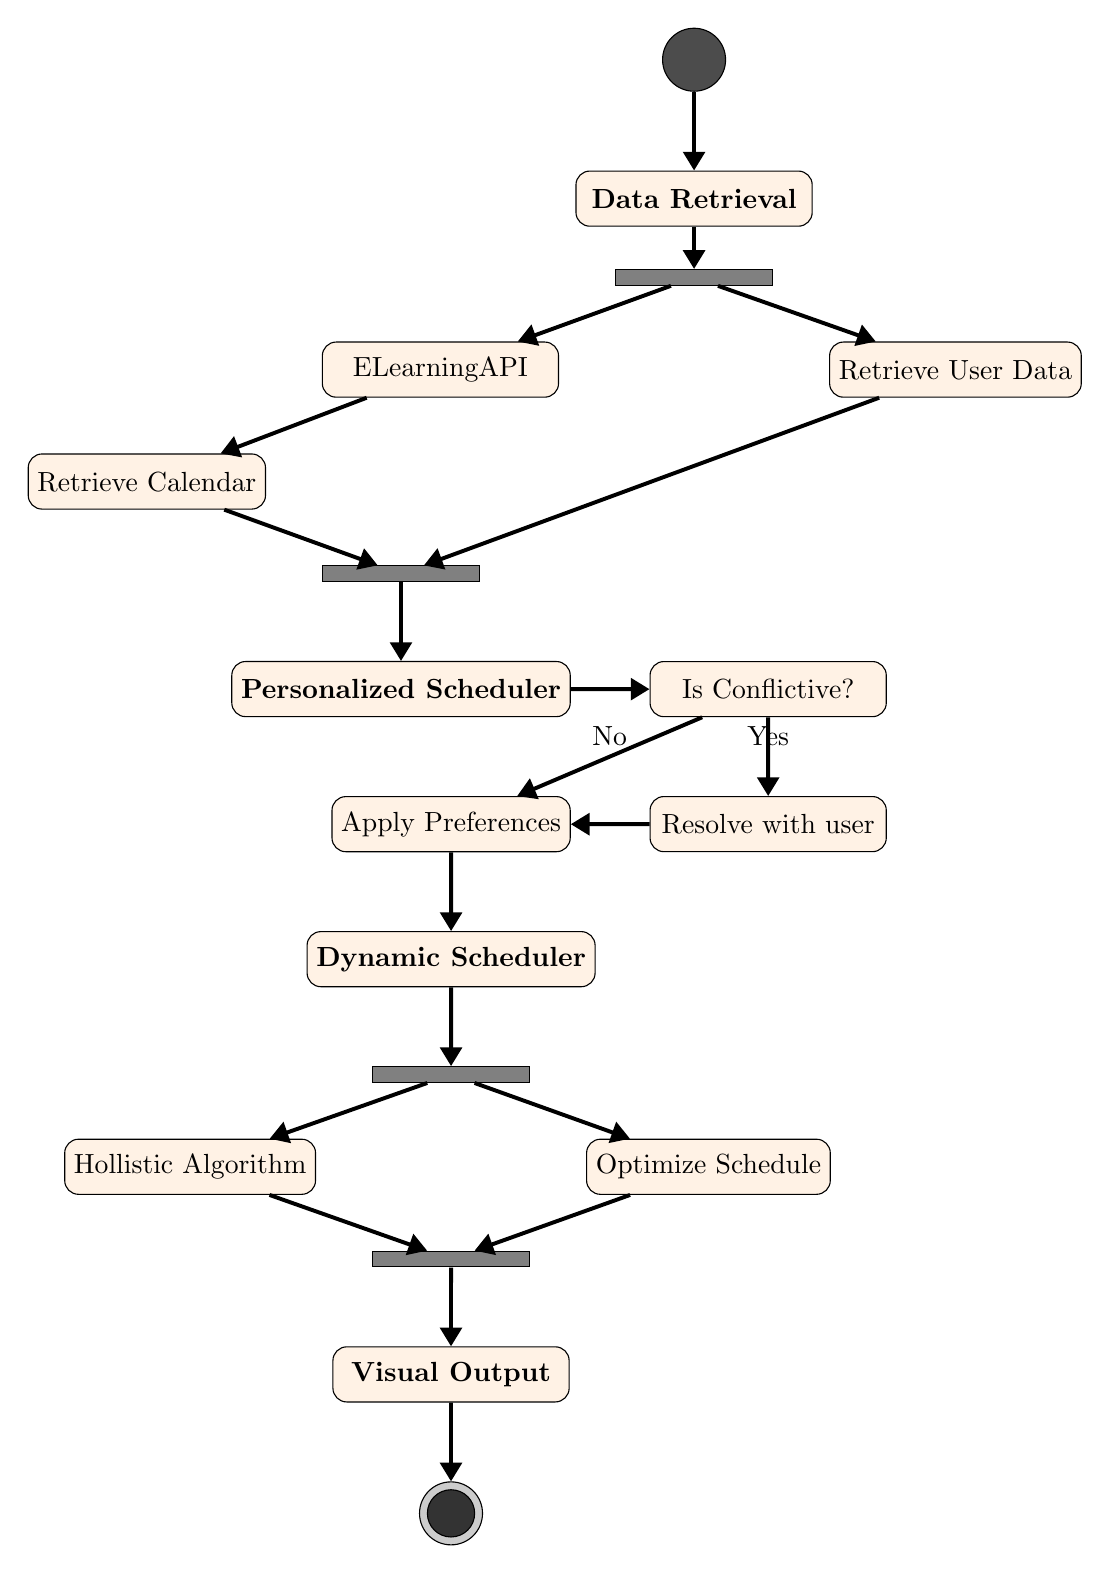
\begin{tikzpicture}[node distance=1cm, scale=0.8]

% Define style for boxes

\tikzstyle{start} = [circle, minimum size=0.8cm, draw=black, fill=black!70]

\tikzstyle{endouter} = [circle, minimum size=0.8cm, draw=black, fill=black!20]
\tikzstyle{endinner} = [circle, minimum size=0.6cm, yshift=-0.1cm, draw=black, fill=black!80]

\tikzstyle{box} = [rectangle, rounded corners=5pt, minimum width=3cm, minimum height=0.7cm, text centered, draw=black, fill=orange!10]

% Define style for arrow
\tikzstyle{arrow} = [thick, -Triangle, line width=0.5mm]

% Define style for fork operation
\tikzstyle{forkstyle} = [rectangle, minimum width=2cm, minimum height=0.2cm, inner sep=0, draw=black, fill=black!50]


% Nodes

% Data Retrieval
\node (start) [start] {};
\node (step1) [below=of start, box] {\textbf{Data Retrieval}};
\node (fork) [below of=step1, forkstyle] {};
\node (step21) [below left=of fork, box] {ELearningAPI};
\node (step31) [below left=of step21, box] {Retrieve Calendar};
\node (step22) [below right=of fork, box] {Retrieve User Data};
\node (fork1) [below right=of step31, forkstyle] {};
% End Data Retrieval

% Personalized scheduler
\node (step41) [below=of fork1, box] {\textbf{Personalized Scheduler}};
\node (step42) [right=of step41, box] {Is Conflictive?};
\node (step51) [below=of step42, box] {Resolve with user};
\node (step52) [left=of step51, box] {Apply Preferences};
% End Personalized scheduler

% Dynamic Scheduler
\node (step61) [below=of step52, box] {\textbf{Dynamic Scheduler}};
\node (fork2) [below=of step61, forkstyle] {};
\node (step71) [below left=of fork2, box] {Hollistic Algorithm};
\node (step72) [below right=of fork2, box] {Optimize Schedule};
\node (fork2end) [below right=of step71, forkstyle] {};

% End Dynamic scheduler

% Start of visual Output
\node (step81) [below=of fork2end, box] {\textbf{Visual Output}};
\node (endo) [below=of step81, endouter] {};
\node (endi) [below=of step81, endinner] {};

% Lines
% Data Retrieval
\draw [arrow] (start) -- (step1);
\draw [arrow] (step1) -- (fork);
\draw [arrow] (fork) -- (step21);
\draw [arrow] (step21) -- (step31);
\draw [arrow] (fork) -- (step22);

\draw [arrow] (step31) -- (fork1);
\draw [arrow] (step22) -- (fork1);
% End Data Retrieval

% Personalized Scheduler
\draw [arrow] (fork1) -- (step41);
\draw [arrow] (step41) -- (step42);
\draw [arrow] (step42) -- (step51) node[midway, above] {Yes};
\draw [arrow] (step42) -- (step52) node[midway, above] {No};
\draw [arrow] (step51) -- (step52);
% End Personalized Scheduler

% Dynamic scheduler
\draw [arrow] (step52) -- (step61);
\draw [arrow] (step61) -- (fork2);
\draw [arrow] (fork2) -- (step71);
\draw [arrow] (fork2) -- (step72);
\draw [arrow] (step71) -- (fork2end);
\draw [arrow] (step72) -- (fork2end);
\draw [arrow] (fork2end) -- (step81);
% End Dynamic Scheduler

\draw [arrow] (step81) -- (endo);
\end{tikzpicture}


\subsection{Data Used}
The \subsystem uses data that is easily identified by how classes interact between each other. Thus, the following UML class chart will help understand the data needed for this subsystem:
\\
\begin{tikzpicture}
    \tikzumlset{fill package=white}
    \tikzumlset{fill class=white}
    \begin{umlpackage}{E-Learning Integration}
        \umlclass{ELearningAPI}{
        } {
            + getCalendar(User) : Calendar \\
            + getData(User) : (Calender, Integer) \\
            + peerData() : (Calender, User, Integer)[]
        }
        
        \umlclass[below=1cm of ELearningAPI]{Calendar}{
            - events : Event \\
        } {
            + getEvents() : Event[]
        }
    \end{umlpackage}

    \begin{umlpackage}{User Profile}
        \umlclass[x=8, y=-2]{User}{
            - username : String \\ 
            - password : String \\ 
            - name : String \\
            - preferences : Preference[] \\
        } {
            + getUsername() : String \\
            + getPassword() : String \\
            + getName() : String \\
            + getPreferences() : Preference[] \\
        }
    \end{umlpackage}

    \begin{umlpackage}{Planning Subsystem}
        \umlclass[x=2, y=-12]{Scheduler}{
            - calendar : Calendar \\
            - user : User \\
        } {
            + generateSchedule() : Schedule \\
        }

        \umlclass[above=1cm of Scheduler]{Schedule}{
            - date : Date \\
            - events : Event[] \\
        } {
            + getDate() : Date \\
            + getEvents() : Event[] \\
        }

        \umlclass[right=1cm of Scheduler]{Preference}{
            - name : String \\
            - value : Integer \\
        } {
            + getName() : String \\
            + getValue() : Integer \\
        }

        \umlclass[above right=1cm of Scheduler ]{Event}{
            - name : String \\
            - duration : Integer \\
        } {
            + getName() : String \\
            + getDuration() : Integer \\
        }
    \end{umlpackage}

    \draw[->] (User Profile.south) -| (Planning Subsystem);
    \draw[->] (E-Learning Integration.south) -| (Planning Subsystem);
\end{tikzpicture}

\newpage



\end{document}
